\section{Referencia de la Clase Busqueda\-Referencia}
\label{classBusquedaReferencia}\index{BusquedaReferencia@{BusquedaReferencia}}
Permite buscar y seleccionar una referencia.  


{\tt \#include $<$busquedareferencia.h$>$}

Diagrama de colaboraci\'{o}n para Busqueda\-Referencia:\begin{figure}[H]
\begin{center}
\leavevmode
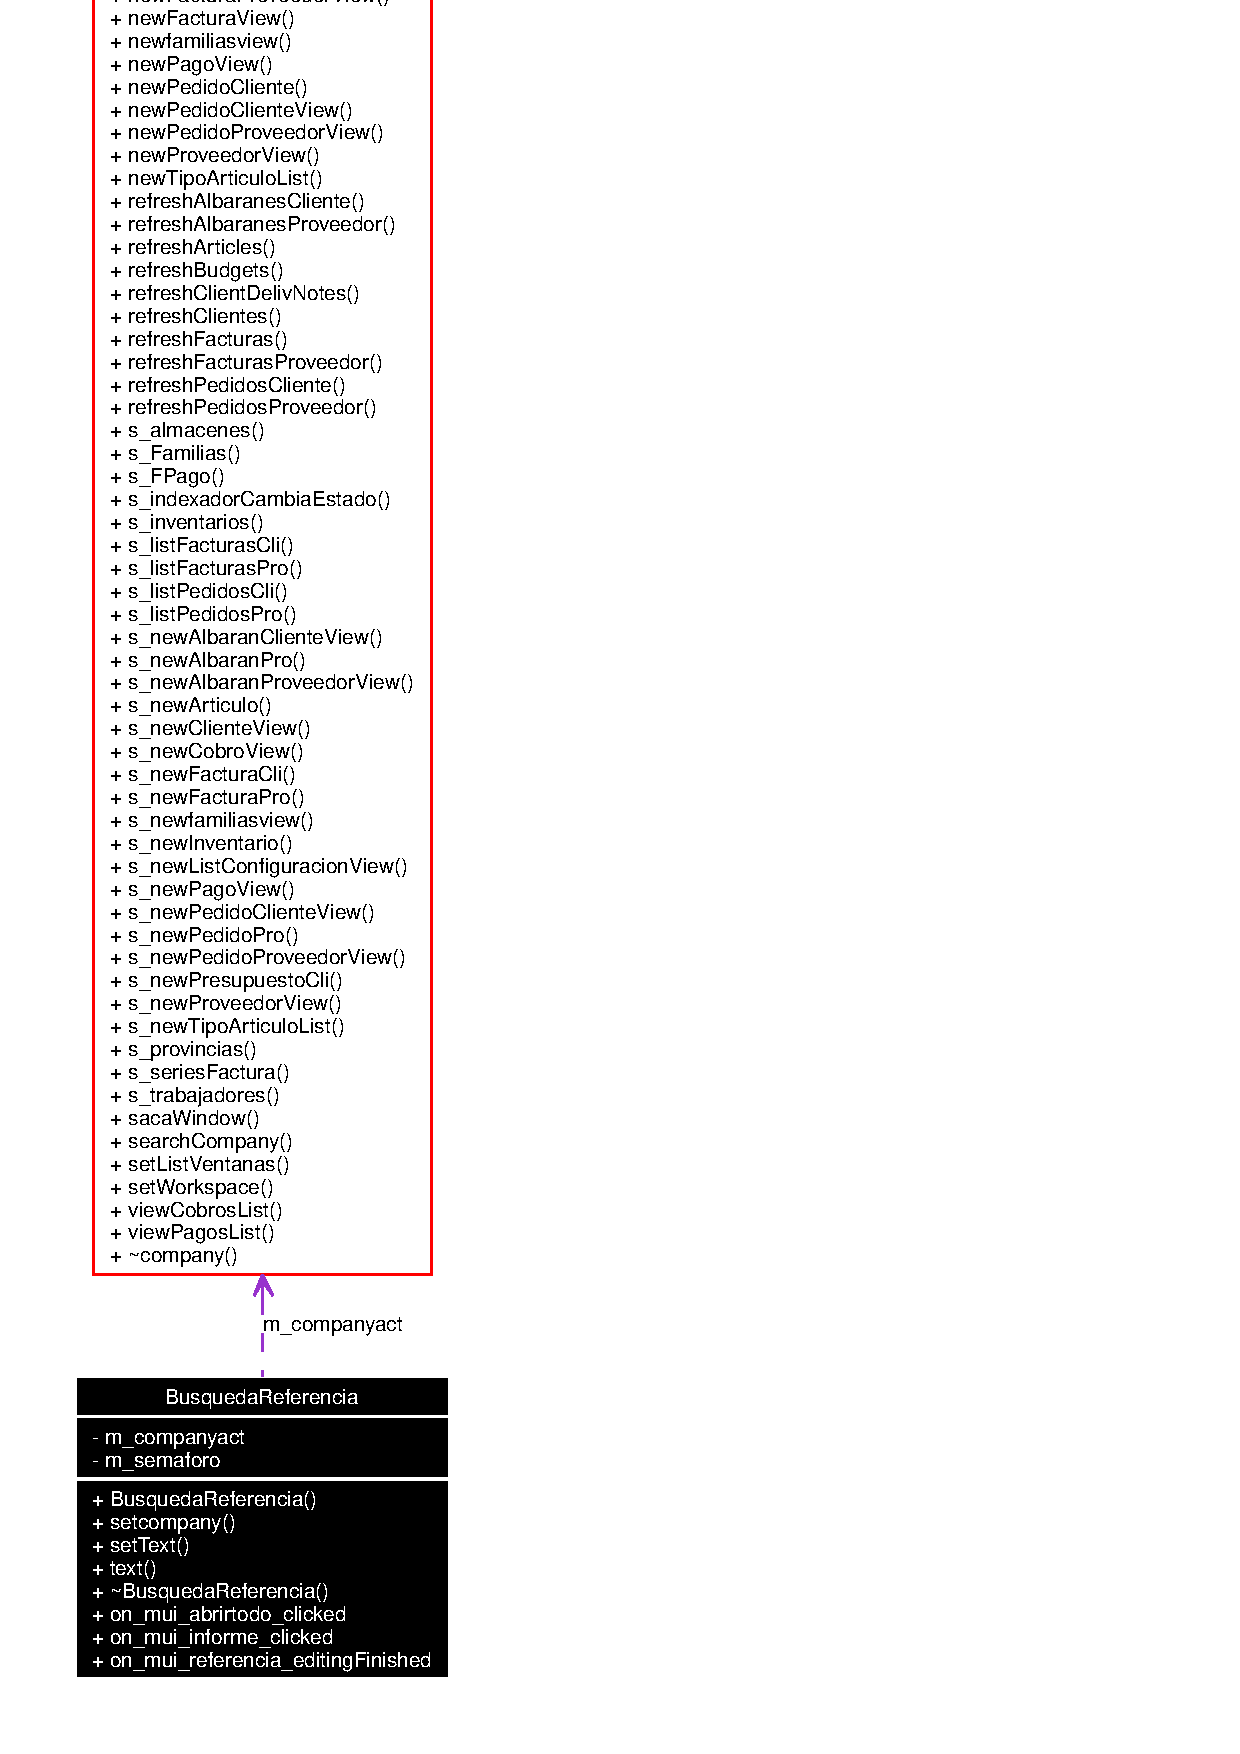
\includegraphics[width=108pt]{classBusquedaReferencia__coll__graph}
\end{center}
\end{figure}
\subsection*{Slots p\'{u}blicos}
\begin{CompactItemize}
\item 
virtual void {\bf on\_\-mui\_\-abrirtodo\_\-clicked} ()
\item 
virtual void {\bf on\_\-mui\_\-informe\_\-clicked} ()\label{classBusquedaReferencia_i1}

\begin{CompactList}\small\item\em B\'{u}squeda de clientes. \item\end{CompactList}\item 
virtual void {\bf on\_\-mui\_\-referencia\_\-editing\-Finished} ()\label{classBusquedaReferencia_i2}

\end{CompactItemize}
\subsection*{Se\~{n}ales}
\begin{CompactItemize}
\item 
void {\bf value\-Changed} (QString)\label{classBusquedaReferencia_l0}

\end{CompactItemize}
\subsection*{M\'{e}todos p\'{u}blicos}
\begin{CompactItemize}
\item 
{\bf Busqueda\-Referencia} (QWidget $\ast$parent=0)\label{classBusquedaReferencia_a0}

\item 
void {\bf setcompany} ({\bf company} $\ast$comp)\label{classBusquedaReferencia_a1}

\item 
virtual void {\bf set\-Text} (QString val)\label{classBusquedaReferencia_a2}

\item 
virtual QString {\bf text} ()\label{classBusquedaReferencia_a3}

\end{CompactItemize}


\subsection{Descripci\'{o}n detallada}
Permite buscar y seleccionar una referencia. 

Muestra la parte del formulario que permite buscar y seleccionar una referencia en cualquier documento. 



\subsection{Documentaci\'{o}n de las funciones miembro}
\index{BusquedaReferencia@{Busqueda\-Referencia}!on_mui_abrirtodo_clicked@{on\_\-mui\_\-abrirtodo\_\-clicked}}
\index{on_mui_abrirtodo_clicked@{on\_\-mui\_\-abrirtodo\_\-clicked}!BusquedaReferencia@{Busqueda\-Referencia}}
\subsubsection{\setlength{\rightskip}{0pt plus 5cm}void Busqueda\-Referencia::on\_\-mui\_\-abrirtodo\_\-clicked ()\hspace{0.3cm}{\tt  [virtual, slot]}}\label{classBusquedaReferencia_i0}


Empezamos con los presupuestos. 

La documentaci\'{o}n para esta clase fu\'{e} generada a partir de los siguientes archivos:\begin{CompactItemize}
\item 
busquedareferencia.h\item 
busquedareferencia.cpp\end{CompactItemize}
